% !TEX root = ../ApproxDA-TransUNet.tex
\section{Experiments}
\label{sec:experiments}

\subsection{Datasets and protocol}
\label{ssec:protocol}

\textbf{Datasets.} \emph{Synapse}~\cite{landman2015miccai}: 30 abdominal CT scans, 8 organs, standard 18/12 train/test split. \emph{Kvasir-SEG}~\cite{jha2020kvasir}: 1000 colonoscopy images with binary polyp masks, using the 880/120 train/test split recommended with the dataset. \emph{ISIC~2018}~\cite{codella2019isic}: dermoscopy images with binary lesion masks, using the official Task~1 training (2594), validation (100), and test (1000) sets.

\textbf{Model selection.} No checkpoint selection is performed: every model, including the re-run DA-TransUNet, is evaluated at its final training epoch, as in TransUNet~\cite{chen2021transunet}. On ISIC~2018, $M$, $r$, $G$, and routing are selected on the official validation set. Synapse and Kvasir-SEG have no validation split; following common practice on Synapse~\cite{chen2021transunet,sun2024datransunet}, their configuration is taken from the ablations in Tables~\ref{tab:window} and~\ref{tab:factors}, which report every configuration on the test set (see Limitations).

\textbf{Training.} All models (including the re-run DA-Trans\-UNet) are trained for 300 epochs with ImageNet-21K pretrained R50-ViT-B/16 weights, $224{\times}224$ input, random rotation and flipping, batch size 24, polynomial learning-rate decay, and loss $\tfrac12\mathcal{L}_{\mathrm{CE}}+\tfrac12\mathcal{L}_{\mathrm{Dice}}$, on the same hardware (\tbd{one NVIDIA Tesla T4}). Following DA-TransUNet~\cite{sun2024datransunet}, Synapse uses SGD (learning rate 0.01, momentum 0.9, weight decay $10^{-4}$) and Kvasir-SEG and ISIC~2018 use Adam (learning rate $10^{-3}$, weight decay $10^{-4}$). We train longer than the original protocols (150 epochs on Synapse; 500 and 50 epochs on Kvasir-SEG and ISIC~2018) and use $224{\times}224$ instead of $256{\times}256$ input on all datasets, so that the same window sizes $M$ apply everywhere. Unless stated otherwise, ApproxDA-TransUNet uses $r{=}32$ and PAM-only routing; $G$ ($=8$ by default) only matters for routings that use CAM.

\textbf{Metrics.} Synapse: mean Dice (DSC) and 95\% Hausdorff distance (HD95, mm) over the 8 organs. Kvasir-SEG and ISIC~2018: DSC and mean IoU (mIoU); we do not report HD95 in mm for these datasets because pixel spacing is not calibrated. \todo{main comparison: mean $\pm$ std over 3 seeds.}

\subsection{Main results}
\label{ssec:main}

\begin{table}[t]
  \caption{Segmentation results. Rows marked $^\dagger$ are values reported in the literature under their original protocols and are shown for reference only; the matched comparison is between the last two rows.}
  \label{tab:main}
  \centering
  \footnotesize
  \setlength{\tabcolsep}{2.2pt}
  \begin{tabular}{@{}lcccccc@{}}
    \toprule
    & \multicolumn{2}{c}{Synapse} & \multicolumn{2}{c}{Kvasir-SEG} & \multicolumn{2}{c}{ISIC 2018} \\
    \cmidrule(lr){2-3}\cmidrule(lr){4-5}\cmidrule(lr){6-7}
    Method & DSC$\uparrow$ & HD95$\downarrow$ & DSC$\uparrow$ & mIoU$\uparrow$ & DSC$\uparrow$ & mIoU$\uparrow$ \\
    \midrule
    U-Net$^\dagger$~\cite{ronneberger2015unet}      & 76.85 & 39.70 & 88.22 & 80.12 & 87.22 & 81.14 \\
    U-Net++$^\dagger$~\cite{zhou2018unetpp}         & 76.91 & 36.93 & 86.57 & 77.67 & 87.30 & 81.33 \\
    Res-UNet$^\dagger$~\cite{diakogiannis2020resunet} & 76.95 & 38.44 & 77.85 & 66.04 & 83.32 & 76.51 \\
    MultiResUNet$^\dagger$~\cite{ibtehaz2020multiresunet} & 77.42 & 36.84 & -- & -- & -- & -- \\
    Att-UNet$^\dagger$~\cite{oktay2018attention}    & 77.77 & 36.02 & 86.61 & 78.01 & 87.60 & 81.51 \\
    \midrule
    TransUNet$^\dagger$~\cite{chen2021transunet}    & 77.48 & 31.69 & 87.91 & 80.03 & 88.78 & 82.63 \\
    UCTransNet$^\dagger$~\cite{wang2022uctransnet}  & 78.23 & 26.75 & --    & --    & --    & --    \\
    TransNorm$^\dagger$~\cite{azad2022transnorm}    & 78.40 & 30.25 & --    & --    & --    & --    \\
    MIM$^\dagger$~\cite{wang2022mim}                & 78.59 & 26.59 & --    & --    & --    & --    \\
    Swin-Unet$^\dagger$~\cite{cao2022swinunet}      & 79.13 & 21.55 & --    & --    & --    & --    \\
    DA-TransUNet$^\dagger$~\cite{sun2024datransunet} & 79.80 & 23.48 & 88.47 & --    & 88.88 & 82.78 \\
    \midrule
    DA-TransUNet (re-run)                            & \tbd{--} & \tbd{--} & \tbd{88.44} & \tbd{81.70} & \tbd{88.43} & \tbd{80.68} \\
    ApproxDA-TransUNet                               & \tbd{80.94} & \tbd{27.49} & \tbd{90.17} & \tbd{84.27} & \tbd{89.55} & \tbd{--} \\
    \bottomrule
  \end{tabular}
  \\[2pt]
  \raggedright\scriptsize ApproxDA-TransUNet: PAM-only routing, $r{=}32$; $M$ = \tbd{Synapse 28, Kvasir-SEG 56, ISIC 2018 28}, selected from the ablations (Synapse, Kvasir-SEG) or on the validation set (ISIC 2018).
\end{table}
% NOTE (remove before submission): current red numbers come from single-seed
% BIBM runs whose checkpoint was selected on the TEST set (val_interval>0,
% _validate_* reads the test split). Existing DA-TransUNet Synapse re-run
% scored 72.03 DSC / 72.52 HD95 (results/DA-TransUNet/Synapse) -- far below the
% reported 79.80; must be investigated before filling the re-run row.
% ISIC ApproxDA M=28 (89.55) is the best in-training test DSC; no separate
% test run / mIoU exists (last epoch ~89.44).

\begin{figure}[t]
  \centering
  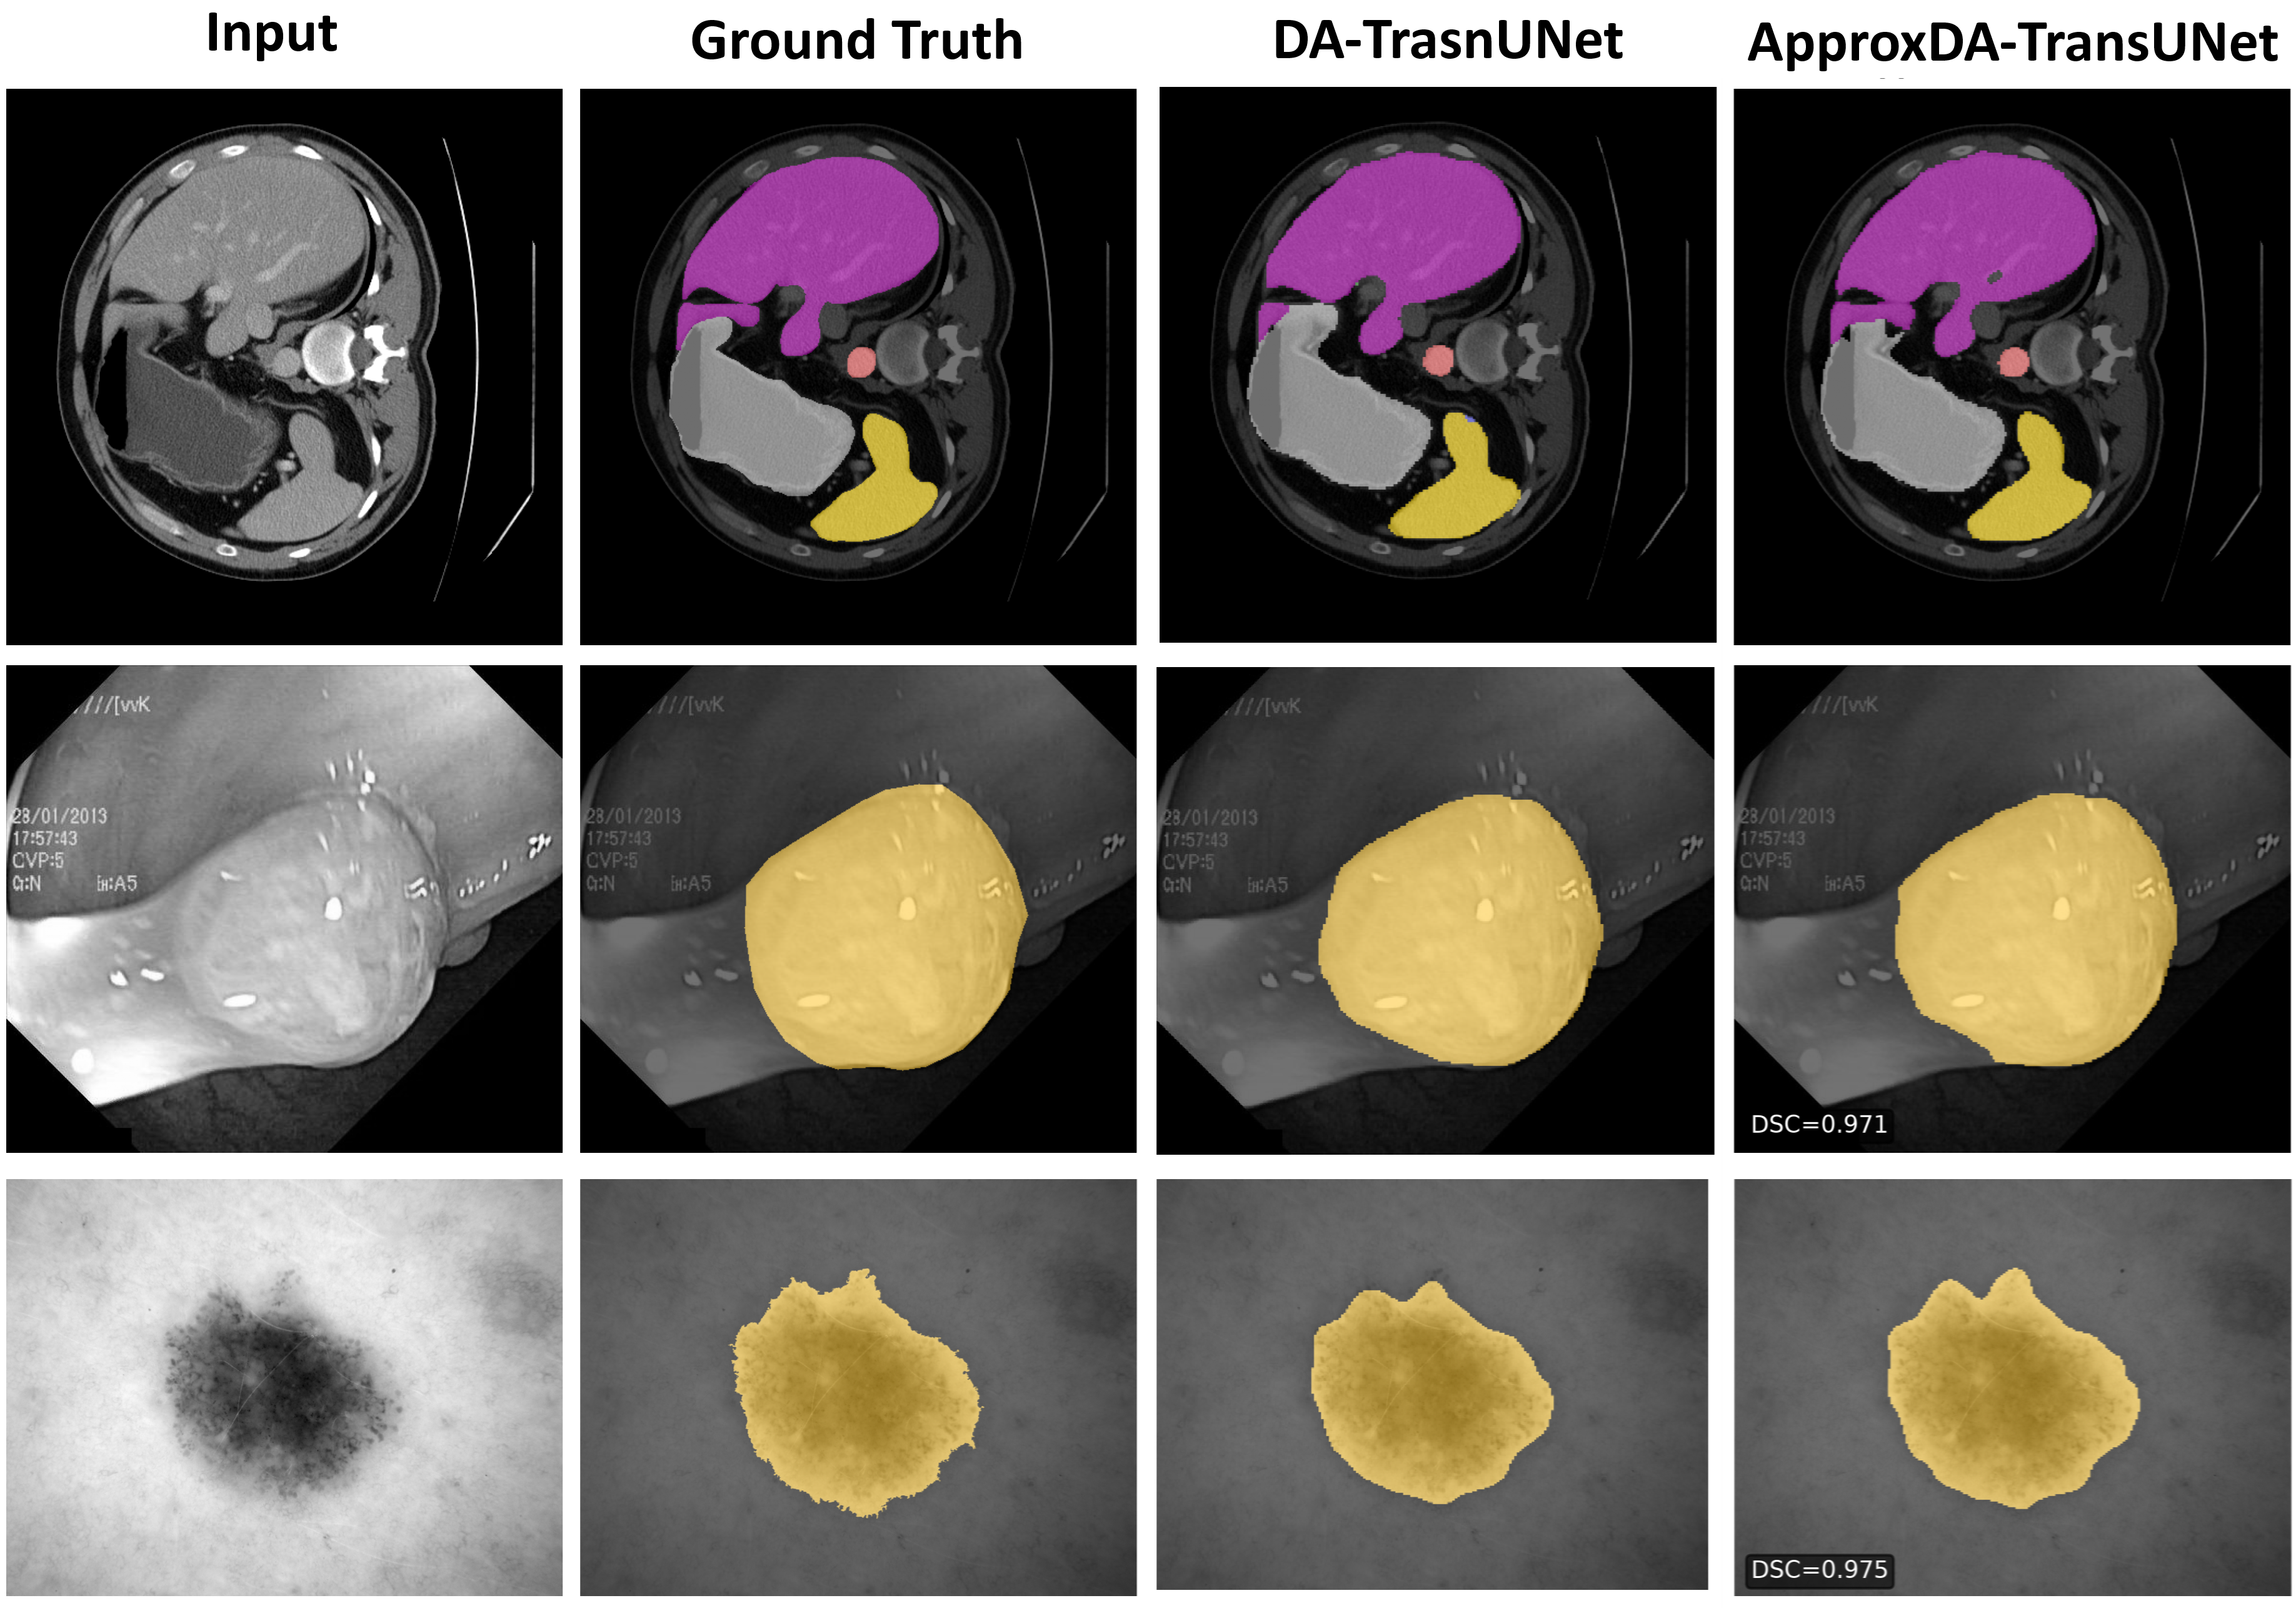
\includegraphics[width=\columnwidth]{figures/fig_qualitative_cross_task.png}
  \caption{Qualitative comparison (columns: input, ground truth, DA-TransUNet, ApproxDA-TransUNet). Top: Synapse ($M{=}\tbd{28}$); middle: Kvasir-SEG ($M{=}\tbd{56}$); bottom: ISIC~2018 ($M{=}\tbd{28}$).}
  \label{fig:qualitative}
\end{figure}
% TODO(figure): regenerate with the re-run (c16, validation-selected) checkpoints
% via experiments/ApproxDA-TransUNet/generate_qualitative_figure.py; the current
% image uses the BIBM legacy checkpoints (and ISIC row used gate=learn, M=7).

Under matched evaluation, ApproxDA-TransUNet improves DSC over the re-run DA-TransUNet on \tbd{all three} datasets (Table~\ref{tab:main}, Fig.~\ref{fig:qualitative}; \tbd{$+1.73$} Kvasir-SEG, \tbd{$+1.12$} ISIC~2018, \todo{Synapse after re-run}). Gains are metric-specific: Synapse HD95 is \tbd{worse} than the reported DA-TransUNet and Swin-Unet values, and ISIC~2018 mIoU is \tbd{below} the reported DA-TransUNet value. \todo{per-organ Synapse DSC; paired test / bootstrap CI (experiments/statistical\_validation.py).}

\subsection{Window sensitivity}
\label{ssec:window}

\begin{table}[t]
  \caption{DSC (\%) versus window size $M$ (PAM-only routing, $r{=}32$). Range $=\max_M \mathrm{DSC}(M) - \min_M \mathrm{DSC}(M)$.}
  \label{tab:window}
  \centering
  \footnotesize
  \setlength{\tabcolsep}{5pt}
  \begin{tabular}{@{}lccc@{}}
    \toprule
    Setting & Synapse & Kvasir-SEG & ISIC 2018 \\
    \midrule
    $M{=}7$                 & \tbd{78.64} & \tbd{89.53} & \tbd{89.41} \\
    $M{=}28$                & \tbd{\textbf{80.94}} & \tbd{89.54} & \tbd{\textbf{89.55}} \\
    $M{=}56$                & \tbd{78.90} & \tbd{\textbf{90.17}} & \tbd{89.05} \\
    $M{=}112$ (global, low-rank) & \tbd{79.44} & \tbd{89.56} & \tbd{89.51} \\
    \midrule
    Range                   & \tbd{2.30} & \tbd{0.64} & \tbd{0.50} \\
    \midrule
    DA-TransUNet (full DA, re-run) & \tbd{--} & \tbd{88.44} & \tbd{88.43} \\
    \bottomrule
  \end{tabular}
\end{table}

Table~\ref{tab:window} varies only $M$. On Synapse, DSC peaks at an intermediate window ($M{=}28$) and drops on both sides (range \tbd{2.30}); Kvasir-SEG and ISIC~2018 are \tbd{3.6--4.6}$\times$ less sensitive (\tbd{0.64} and \tbd{0.50}). We call this range the \emph{empirical window sensitivity}; it describes a model's response to $M$ on a dataset, not an independent predictor of contextual requirement. The difference is consistent with multi-organ CT depending more on inter-organ context than polyp and lesion segmentation, which depend mainly on local appearance. The sensitivity also bounds how much the choice of $M$ matters in practice: on Kvasir-SEG and ISIC~2018 any tested window stays within \tbd{0.64} points of the best, whereas on Synapse the window must be tuned. On all three datasets the best window \tbd{exceeds} DA-TransUNet, suggesting a locality-induced bias. This comparison changes both the attention approximation and the routing (PAM-only instead of PAM + CAM); the exact-PAM row of Table~\ref{tab:factors} isolates the approximation itself. $M{=}112$ keeps the rank-32 projection and thus differs from full PAM.

Fig.~\ref{fig:attn_map} visualizes this bias on Kvasir-SEG. On 10 test images, windowed PAM ($M{=}7$) places $62.3\%$ of its contribution inside the polyp region, compared with $34.2\%$ for global PAM ($M{=}112$), and the windowed share is higher in 9 of the 10 images. Windowed attention concentrates on polyp boundaries, whereas global attention spreads over surrounding tissue. This observation is consistent with the locality interpretation but does not by itself establish a causal link to accuracy.

\begin{figure}[t]
  \centering
  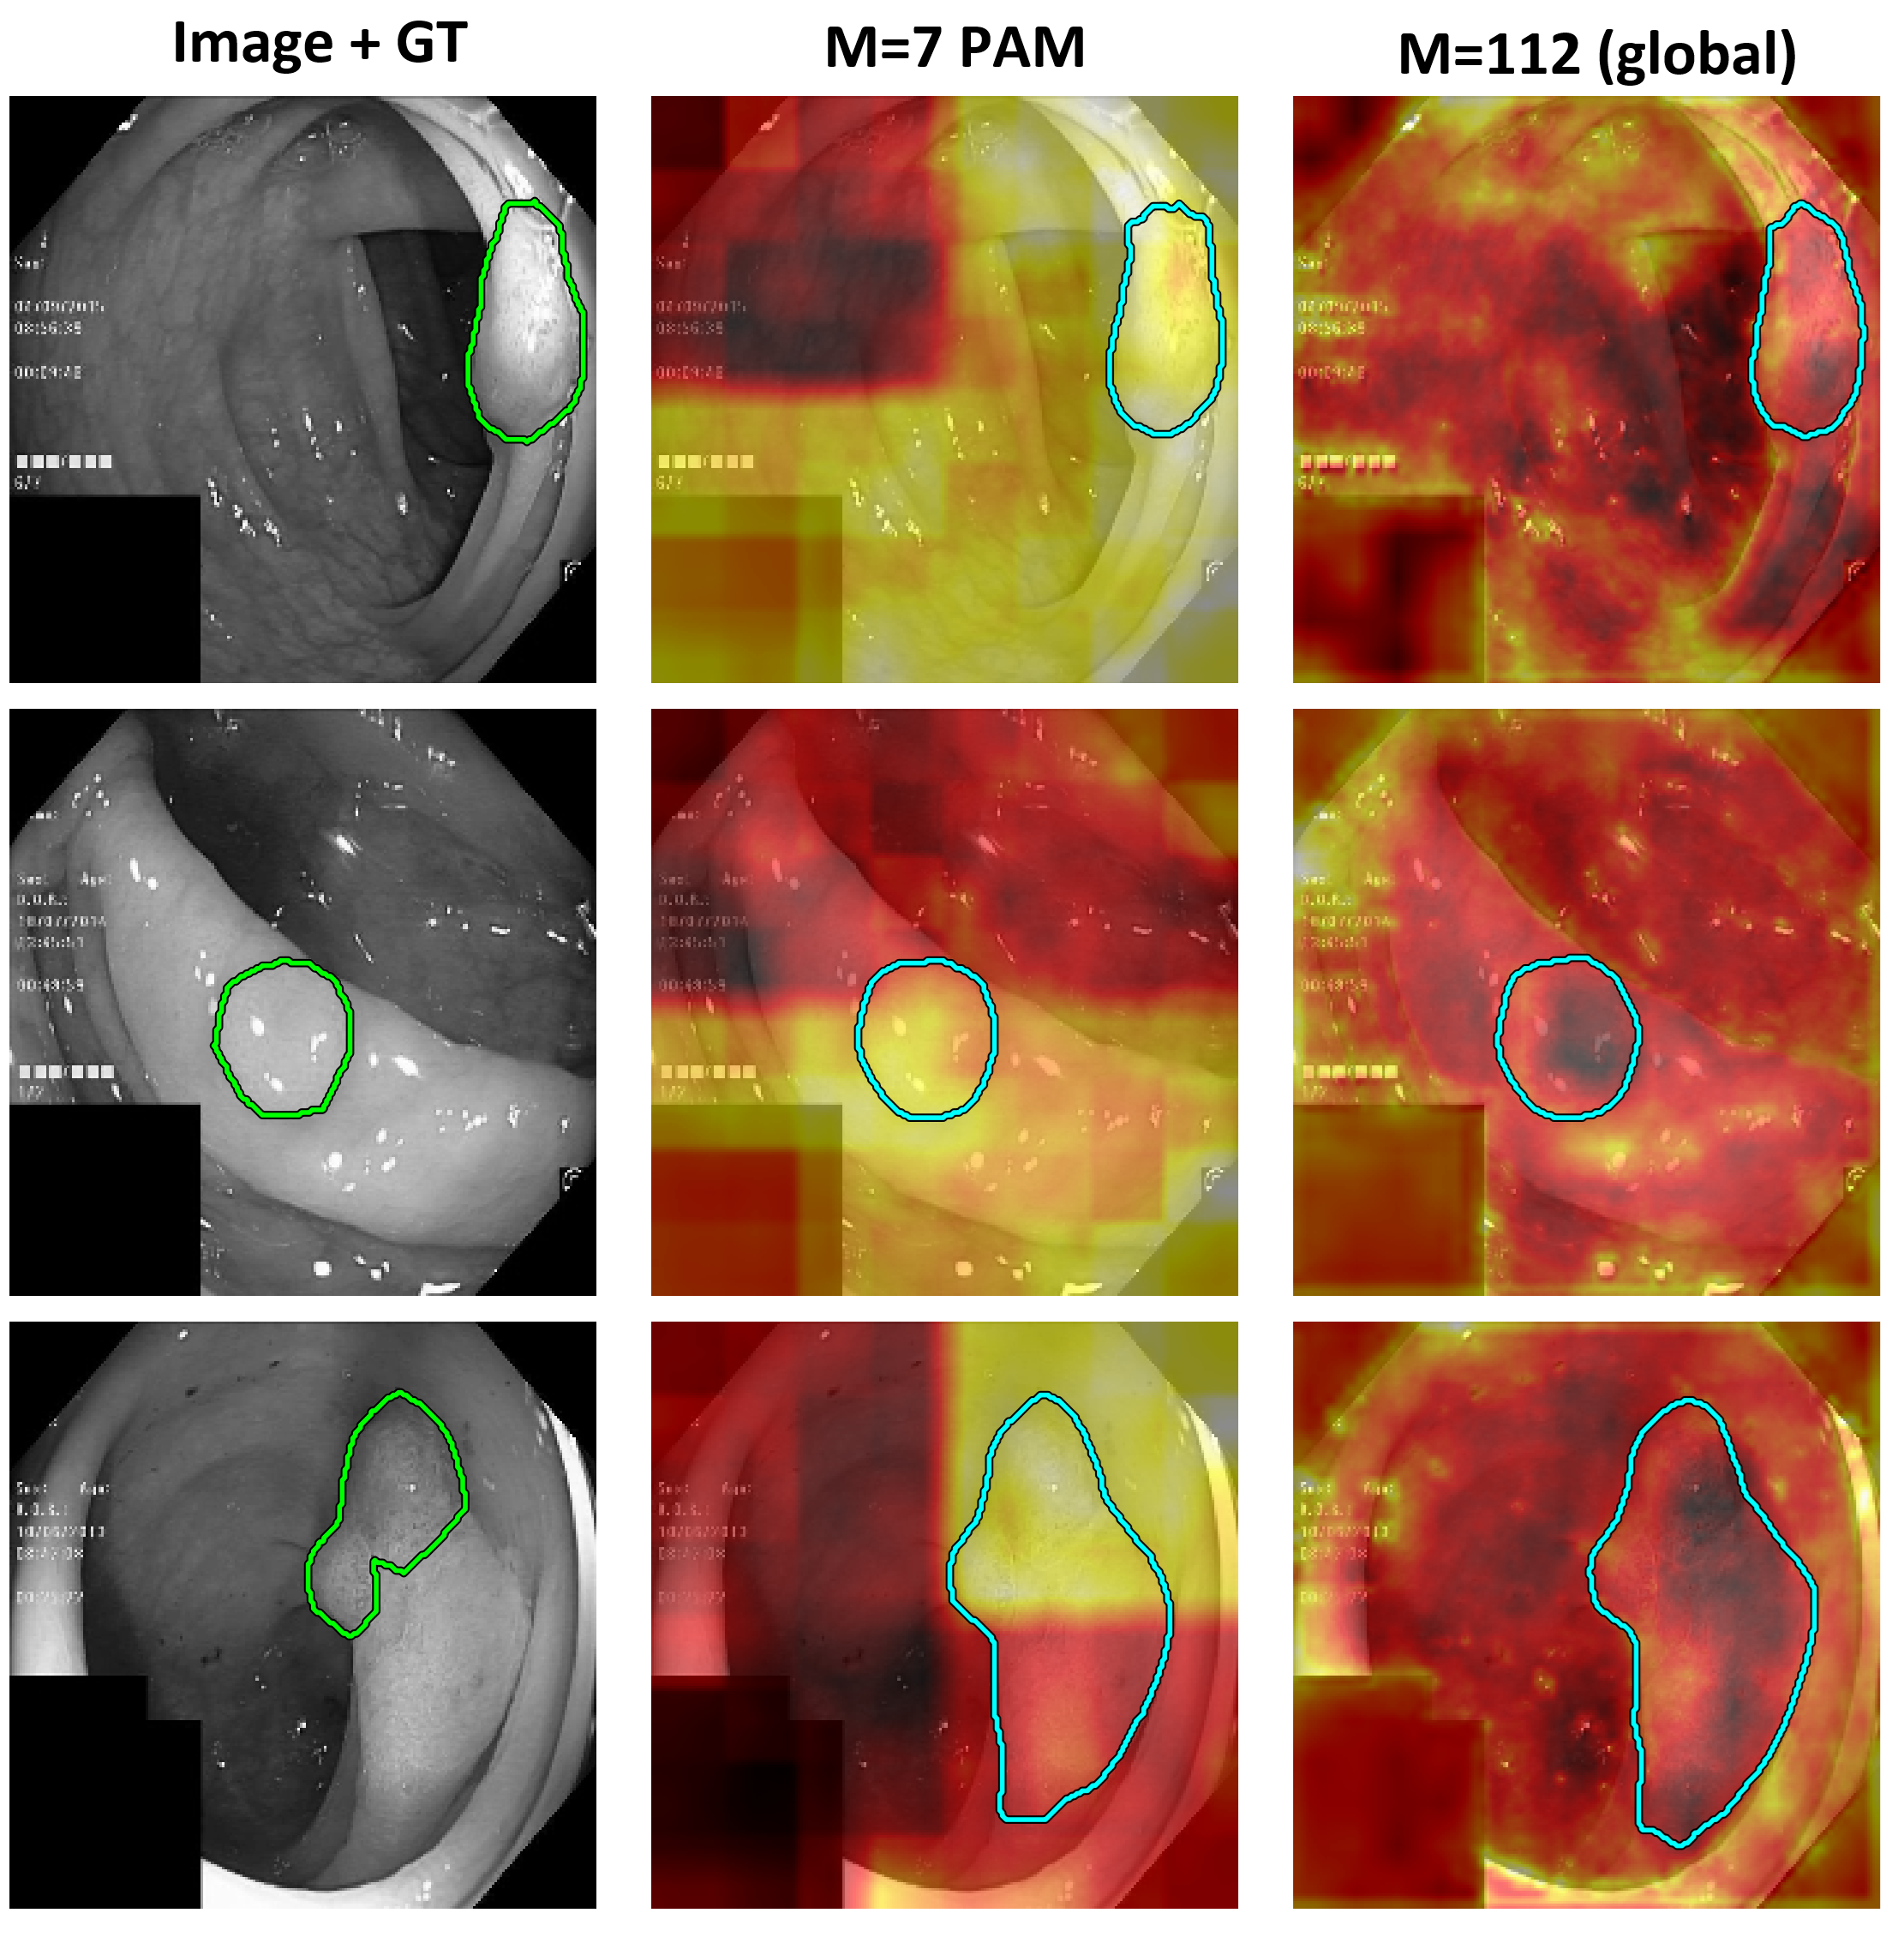
\includegraphics[width=\columnwidth]{figures/attn_Kvasir_M7_r32_pam_vs_M112.png}\\[-4pt]
  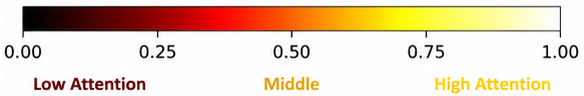
\includegraphics[width=0.68\columnwidth]{figures/hot_color_code.png}
  \caption{PAM contribution maps ($\|\text{output}-\text{input}\|_2$) on three Kvasir-SEG images. Each row: input with ground-truth contour (left), windowed PAM with $M{=}7$ (center), global PAM with $M{=}112$ (right). Each panel is normalized independently, so magnitudes are not comparable across panels.}
  \label{fig:attn_map}
\end{figure}

\subsection{Rank, grouping, and routing}
\label{ssec:factors}

\begin{table}[t]
  \caption{Single-factor ablations on Synapse. Each block varies one factor; the others are fixed as indicated.}
  \label{tab:factors}
  \centering
  \footnotesize
  \setlength{\tabcolsep}{4pt}
  \begin{tabular}{@{}llcc@{}}
    \toprule
    Factor (fixed) & Setting & DSC$\uparrow$ & HD95$\downarrow$ \\
    \midrule
    \multirow{4}{*}{\shortstack[l]{Rank $r$\\($M{=}112$, PAM)}} & $r{=}16$ & \tbd{--} & \tbd{--} \\
                                   & $r{=}32$ & \tbd{79.44} & \tbd{27.26} \\
                                   & $r{=}64$ & \tbd{78.93} & \tbd{31.21} \\
                                   & no projection & \tbd{--} & \tbd{--} \\
    \midrule
    \shortstack[l]{Window only\\($M{=}28$, PAM)} & no projection & \tbd{--} & \tbd{--} \\
    \midrule
    \multirow{3}{*}{\shortstack[l]{Groups $G$\\(CAM-only)}} & $G{=}1$ & \tbd{--} & \tbd{--} \\
                                   & $G{=}4$ & \tbd{--} & \tbd{--} \\
                                   & $G{=}8$ & \tbd{78.26} & \tbd{30.59} \\
    \midrule
    \multirow{4}{*}{\shortstack[l]{Routing\\($M{=}7$, $r{=}32$)}} & PAM-only & \tbd{78.64} & \tbd{31.09} \\
                                   & CAM-only & \tbd{78.26} & \tbd{30.59} \\
                                   & fixed $g{=}0.5$ & \tbd{--} & \tbd{--} \\
                                   & learned & \tbd{77.78} & \tbd{34.29} \\
    \bottomrule
  \end{tabular}
\end{table}
% NOTE: Groups block -- in PAM-only routing the CAM branch output is discarded,
% so G has no effect there; the G ablation therefore uses CAM-only routing
% (M irrelevant). G=8 row = existing M7R32-CAM run.

In Table~\ref{tab:factors}, raising $r$ from 32 to 64 does \tbd{not} improve DSC, so window scale matters more than rank in the tested range; the no-projection row is exact global PAM (PAM-only routing), isolating the effect of the approximation from that of the routing, and the window-only row removes the projection at the best Synapse window. $G$ is ablated under CAM-only routing, since CAM does not contribute under PAM-only routing. \todo{grouping result.} The learned gate converged to $g \approx 0.5$ in our Synapse experiments and did not outperform PAM-only routing, which we therefore use elsewhere.

\textbf{Limitations.} Because Synapse and Kvasir-SEG have no validation split, their configurations were selected from test-set ablations, so the reported ApproxDA-TransUNet results on these datasets may be optimistic. The bias is bounded by the window-sensitivity range: small on Kvasir-SEG (\tbd{0.64} points), but up to \tbd{2.30} points on Synapse, where fine window selection is precisely what our results call for; in practice, $M$ should be tuned on held-out data. We also use three datasets and one backbone, and whether window sensitivity can be predicted without window ablations remains open.
